\documentclass[conference]{IEEEtran}
\usepackage{amsmath,amssymb,amsfonts}
\usepackage[utf8]{inputenc}
\usepackage{url}
\usepackage{subfigure}
\usepackage{booktabs,threeparttable,multirow}
\usepackage{graphicx}
\usepackage{hyperref}
\usepackage[ngerman]{babel}

% new math operators
\DeclareMathOperator{\abs}{abs}

% todo command
\usepackage{marginnote}
\newcounter{todocnt}
\setcounter{todocnt}{0}
\newcommand{\todo}[1]{\stepcounter{todocnt}{\tt {[#1]}} \marginpar{{$\blacksquare$ \thetodocnt}}}  
\newcommand{\specialcell}[2][c]{%
  \begin{tabular}[#1]{@{}c@{}}#2\end{tabular}}

\hyphenation{op-tical net-works semi-conduc-tor}
\IEEEoverridecommandlockouts
\begin{document}

\title{Projekt: Rowhammer}


\author{\IEEEauthorblockN{Gilian Henke\\ Dominik Mairhöfer}
\IEEEauthorblockA{University of Lübeck\\
Email: \texttt{gilian.henke@student.uni-luebeck.de}\\ \texttt{dominik.mairhoefer@student.uni-luebeck.de}}}
\maketitle

\begin{abstract}
Das Ziel des Projekts ist es einen One-Location Rowhammer Angriff nach dem Paper \cite{DBLP:journals/corr/abs-1710-00551} zu implementieren. Dieser Angriff soll dann verwendete werden, um lokal die Rechte zu erweitern. Dafür soll unter anderem auch die neue Methode des Memory chasing verwendet werden.\\
Beim hierbei zu Grunde liegenden Modell, kann die Software Schutzmechanismen besitzen, aber nicht die Hardware. Der Angreifer kann ein arbiträres, unprivilegiertes Programm starten. Unter diesen Voraussetzungen kann der Angriff durchgeführt werden.


\end{abstract}

\section{Motivation}
\todo{Know what you want to do and why that is interesting (maybe with bullet points). But do not write this section until you know what you actually have done so that the motivation fits your work. Aus diesen genannten Gründen noch nicht geschrieben.}


We will stick to the following timeline: (Zur Orientierung beibehalten)

\begin{itemize}
	\item 12/18:  Submission of motivation, background, project scope and related work: please give a description of the technical aspect of your work, i.e. detailed background description of attacks. Also describe related work and outline, in more detail, your technical steps.
	\item 1/15: First version of report. This should be ver close to the final version, only technical parts that have not yet been finished should be missing.
	\item 2/1 : Final submission of complete project description.
	\item 2/8: Project Presentations in class: 25 minutes presentation plus questions. 
\end{itemize}

\section{Hintergrund}\label{sec:background}
Die hier betrachteten Rowhammer Angriffe basieren auf folgendem Modell. Das System, auf welchem der Angriff ausgeführt werden soll, besitzt keine Maßnahmen der Hardware, um Rowhammer Angriff zu entdecken und zu unterbinden. Die verwendete Software darf jedoch versuchen, zu erkennen, ob ein Angriff stattfindet, und jenen zu verhindern. Damit solch ein Angriff überhaupt ausgeführt werden kann, muss der Angreifer in der Lage sein, ein beliebiges, nicht privilegiertes Programm auf dem System zu starten.\\
Im Folgendem werden dann die Methoden beschrieben, mit denen ein Rowhammer Angriff ausgeführt werden kann. Im Rahmen dieses Projekts wird dann versucht, einen Teil dieser Methoden anzuwenden und zu implementieren.
\subsection{Überblick über den Angriffsablauf}
Der in dem Paper beschriebene Angriff lässt sich in mehrere einzelne Schritte unterteilen. Diese laufen in der folgenden Reihenfolge ab:
\begin{enumerate}
	\item One-Location Rowhammer \\
	Zuerst wird durch einen One-Location Rowhammer Angriff versucht wahllos Bits im Speicher zu flippen. Dies dient dazu, Adressen im virtuellen Adressbereich zu finden, für die es überhaupt möglich ist Bits zu flippen.
	
	\item Prefetch Side-Channel Attack \\
	Anschließend werden mit Hilfe einer Prefetch Side-Channel Attacke die physikalischen Adressen zu den im ersten Schritt gefundenen virtuellen Adressen herausgefunden.
	
	\item Memory Waylaying \& Prefetch Side-Channel Attack \\
	Um ein Bit in einer Datei zu flippen, für die es keine Schreibrechte gibt, wird diese in den Arbeitsspeicher geladen. Mit Memory Waylaying wird sie immer wieder an unterschiedliche Adressen geladen. Nach jedem neuen Laden wird mit der Prefetch Side-Channel Attacke die physikalische Adresse herausgefunden, an die die Datei geladen wurde.
	Wurde die Datei an eine physikalische Adresse geladen, für die in den ersten beiden Schritten herausgefunden wurde, dass sie für einen One-Location Rowhammer Angriff verwundbar ist, wird mit dem nächsten Schritt fortgefahren.
	
	\item One-Location Rowhammer
	Da die Datei nun an einer bekannten Adresse liegt, kann der  One-Location Rowhammer Angriff aus dem ersten Schritt für diese Adresse erneut ausgeführt werden. Damit wird ein Bit an der physikalischen Adresse geflippt und man erhält eine veränderte Datei.
\end{enumerate}

Im folgenden werden die einzelnen Schritte genauer beschrieben.

\subsection{Memory Waylaying}
In dem Paper werden zwei neue Methoden vorgestellt, um eine Seite an einer bestimmten physikalischen Adresse im Arbeitsspeicher zu platzieren. Dieser Prozess nennt sich Memory Waylaying. Hierbei wird im Gegensatz zu anderen Methoden nicht der gesamte Speicher mit Daten gefüllt, was die Entdeckung schwieriger macht. Das dies möglich ist, beruht darauf, dass, wenn Daten, wenn sie aus dem DRAM entfernt werden, beim Laden an eine zufällige Adresse platziert werden. Durch wiederholtes Anwenden dieser Methode kann die Seite an die richtige Position im Speicher positioniert werden.\\
 Mit Hilfe eines Prefatch-based Prediction Oracle, näher beschrieben in \cite{DBLP:conf/ccs/2016}, kann dann überprüft werden, ob zwei virtuelle Adressen, auf die gleiche physikalische verweisen. Damit kann dann überprüft werden, ob eine Seite an einer bestimmten Stelle im Speicher liegt. Dieses Orakel besteht aus zwei Schritten. Zunächst der prefatch und dann eine Flush and Reload Attacke. \\
Um das Memory Waylaying durchzuführen, müssen zunächst die Pages aus dem Cache entfernt werden, damit sie bei einem erneuten Zugriff eine neue physische Adresse erhalten. Man könnte diese Pages einfach entfernen, in dem man einfach eine genügend große Menge an Speicher allokiert. Dies kann aber zu Systemfehlern durch Mangel an Speicher erzeugen. Dementsprechend wird versucht eine bessere Möglichkeit zu finden. Man kann dies optimieren, indem man das Wissen hinzunimmt, dass nicht ausführbare Pages eher als ausführbare entfernt werden und ausführbare eher als ausführbare mit lesendem Zugriff. Außerdem muss man wissen, wann die zu entfernende Page nicht mehr im Cache ist. Dazu kann man entweder genügend Pages entfernen, sodass die Wahrscheinlichkeit groß genug ist, oder man kann überprüfen, zum Beispiel mit \texttt{mincore} unter Linux, ob die Page noch im Cache ist. Hierbei muss man abwägen, ob Geschwindigkeit oder Nichtaufdeckbarkeit wichtiger ist.\\
Zusammen mit dem Prefatch-based Prediction Oracle kann man dann das Memory Waylaying durchführen und überprüfen, ob die Page an der richtigen Stelle positioniert ist. Die korrekte Position ist eine, von der man weiß, dass man hier einen Bitflip erzeugen kann.\\
Der komplette Prozess des Memory Waylaying kann Laufzeiten von 100 Stunden benötigen. Daher gibt es eine effizientere Variante, das Memory Chasing. Beim Memory Chasing wird der copy-on-write Effekt des \textit{fork}-Befehls ausgenutzt. Dazu nehmen wir eine Page, die wir an eine bestimmte Stelle positionieren wollen und setzen sie als \texttt{private} und \texttt{writeable}. Dann verwenden wir \texttt{fork} auf den Prozess. Den dadurch entstehenden \texttt{Child}-Prozess erzeugen wir, damit er dadurch auch tatsächlich an eine neue physische Adresse geschrieben wird. Dies geschieht durch den copy-on-write Effekt des \texttt{fork}. Danach wird der \texttt{Parent}-Prozess entfernt und dann die Prozedur wiederholt bis die Page an der gewünschten Adresse ist.\\

\subsection{One-Location Rowhammer}
Durch die fortschreitende Entwicklung vom DRAM, werden einzelne Speicherzellen mit immer weniger Spannung betrieben. Dies führt jedoch, dazu dass schon geringe Änderungen der Spannung ein Flip eines Bits zur Folge haben können. Dieses Flippen kann man durchs gehäufte, schnelle Zugreifen auf benachbarte Speicherzellen, Hämmern genannt, bewusst auslösen.
 Beim double-sided Rowhammer wird auf beiden Seiten der zu flippenden Speicherreihen gehämmert, während beim single-sided Rowhammer nur eine Seite gehämmert wird. Im Gegensatz zum Namen wird bei diesen Angriffen jedoch mehr als nur eine einzige Speicherzelle gehämmert.\\
Betrachten wir als nächstes den One-Location Rowhammer. Bei dieser Methode wird im Gegensatz zu den üblichen Methoden nur eine einzige Stelle im Speicher gehämmert und dann überprüft, ob im benachbarten Speicher Bitflips aufgetreten sind. Hierbei werden zwar weniger Bitflips erzeugt, aber die Entdeckung ist wesentlich schwieriger. Die Anzahl der hierbei erzeugten Bitflips ist aber immer noch ausreichend, um einen Angriff durchzuführen.\\
Bei der Durchführung dieses Angriffes wird zunächst der zu testende Speicher allokiert und mit zufälligen aber wiedererkennbaren Werten gefüllt. Dann wird durch wiederholtes Hämmern versucht in diesem Speicher ein Bitflip zu erzeugen. Der Einfachheit halber wird bei diesem Angriff immer eine zufällige Adresse gehämmert. Hierbei wird eine Adresse aus dem betrachtetem Speicher zufällig gewählt und dann wird auf jene Adresse wiederholt zugegriffen. Nach jedem Zugriff wird der Wert dieser Adresse jedoch immer wieder aus dem Cache entfernt, zum Beispiel mit \texttt{clflush}, sodass erneut auf den DRAM zugegriffen werden muss. Danach wird überprüft, ob das Hämmern an dieser Adresse irgendeine Veränderung erzeugt hat. Wenn dies eine Veränderung bewirkt hat, dann haben wir unsere Adresse für den Bitflip gefunden. Wenn diese keine Veränderung bewirkt hat, dann wiederholen wir das Hämmern an einer neuen Adresse.\\
Der Vorteil dieses Angriffes gegenüber des double-sided Rowhammer ist, dass er äußerst einfach ist und schwer von herkömmlichen Strategien zu entdecken ist. Der Nachteil hierbei ist es jedoch, dass die Wahrscheinlichkeit für einen Bitflip deutlich geringer ist. Ein weiterer Nachteil ist es, dass man hiermit noch nicht die tatsächliche physikalische Adresse des zu flippenden Speichers erhält, sondern nur dessen virtuelle Adresse.

\subsection{Prefetch Side-Channel Attacke}

Die Prefetch Side-Channel Attacke aus \cite{DBLP:conf/ccs/2016} dient dazu, zu einer virtuellen Adresse die dazugehörige physikalische Adresse herauszufinden. 

Der virtuellen Adressraum jedes Prozesses ist unterteilt in zwei Bereiche. Den User und Kernel Bereich. Ein laufender Prozess im User Modus kann lediglich auf den User Bereich zugreifen und im Kernel Bereich weder lesen noch schreiben. Dies ist nur möglich, wenn die CPU im Kernel-Modus läuft und somit dem Kernel vorbehalten. Trotzdem ist auch der Kernel Bereich im virtuellen Adressraum jedes Prozesses enthalten.

Bei einigen Betriebssystemen, insbesondere beim Linux Kernel \cite{virtual-momory}, findet sich im Kernel Bereich eine Region in welcher der gesamte physikalische Speicher in den virtuellen Adressraum gemappt wird.
Zum Beispiel befindet sich beim Linux Kernel diese Region im virtuellen Adressbereich von \texttt{0xffff880000000000} bis \texttt{0xffffc7ffffffffff}.
Das bedeutet auf die physikalische Adresse \texttt{0x00} kann über die virtuelle Adresse \texttt{0xffff880000000000} zugegriffen werden.

Weiter bedeutet dies auch, dass für jede physikalische Adresse, die über eine virtuelle Adresse aus dem User Bereich angesprochen werden kann, eine weitere virtuelle Adresse im Kernel Bereich existiert, die auf die gleiche physikalische Adresse zeigt. Dies ist in Abbildung \ref{fig:direct-mapping} dargestellt.

\begin{figure}
	\centering
	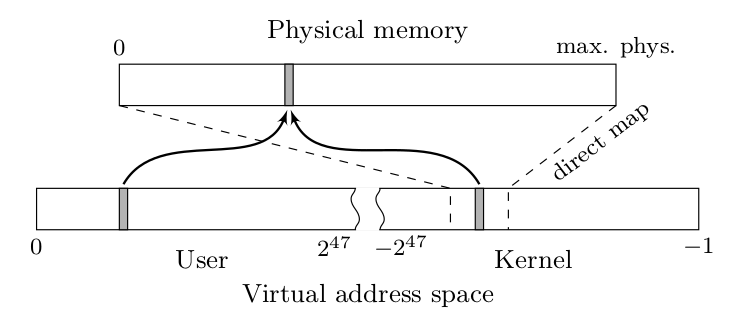
\includegraphics[width=1\linewidth]{direct-mapping}
	\caption{Direktes Mapping des gesammten physikalischen Speichers. Jede pyhsikalische Adresse ist zwei mal vorhanden, einmal im User und Kernel Bereich \cite{DBLP:conf/ccs/2016}}
	\label{fig:direct-mapping}
\end{figure}


Ist für eine virtuelle Adresse aus dem User Bereich die dazugehörige virtuelle Adresse aus dem Kernel Bereich bekannt, lässt sich offensichtlich die physikalische Adresse einfach berechnen, indem von der virtuellen Adresse im Kernel Bereich der Offset \texttt{0xffff880000000000} abgezogen wird. Die Schwierigkeit liegt darin, diese Adresse zu finden. 


Um die passende virtuelle Adresse im Kernel Bereich zu finden kann nun folgende Eigenschaft ausgenutzt werden:

Auf modernen Prozessoren gibt es einen \texttt{prefetch} Befehl, welche die CPU darauf hinweist, dass die Daten unter einer bestimmten Adresse bald benötigt werden. Die CPU lädt diese dann in den Cache, damit sie schneller verfügbar sind. Entscheidend dabei ist, dass man jede Adresse aus dem virtuellen Adressbereich mittels \texttt{prefetch} in den Cache laden kann, auch solche die im Kernel Bereich liegen. Der Cache der CPU beruht jedoch auf physikalischen Adressen. Das bedeutet, wenn eine Adresse in den Cache geladen wird, wird bei jedem Zugriff auf eine virtuelle Adresse die auf die physikalische zeigt, auf den Cache zugegriffen.

Mithilfe des Prefetchings kann nun eine Cache Timing Attacke durchgeführt werden, welche wie folgt abläuft:
\begin{enumerate}
	\item Auf die virtuelle Adresse im User Bereich, zu welche die dazugehörige im Kernel Bereich gefunden werden soll, wird ein \texttt{flush} ausgeführt. Dadurch wird diese aus allen Caches der CPU entfernt. 
	\item Anschließend wird eine virtuelle Adresse aus dem Kernel Bereich mittels eines \texttt{prefetch} in den Cache geladen.
	\item Dann wird lesend auf die Adresse aus dem User Bereich zugegriffen. Erfolgt der Lesezugriff schnell, wurde die Adresse wahrscheinlich zwischendurch in den Cache geladen und die virtuellen Adressen aus User und Kernel Bereich zeigen aus die gleiche physikalische Adresse. Erfolgt der Zugriff langsam ist dies wahrscheinlich nicht der Fall.
\end{enumerate}

Diese Schritte können nun für alle virtuellen Adressen von \texttt{0xffff880000000000} bis \texttt{0xffffc7ffffffffff} wiederholt werden, bis einmal ein schneller Zugriff erfolgt und somit die passende Adresse aus dem Kernel Bereich gefunden wurde.

Um zuverlässig ein korrektes Ergebnis zu erhalten muss im dritten Schritt sehr hochauflösend die Zeit gemessen werden. Dies kann mit Hilfe des \texttt{rdtsc} Befehls erfolgen, mit dem die Anzahl an Clock-Zyklen der CPU gemessen werden können. Nach \cite{DBLP:conf/ccs/2016} liegt die Anzahl der Zyklen bei einem Zugriff auf Cache bei circa 180, und ansonsten bei circa 380.
Weiter muss die Messung für jede zu prüfende Adresse aus dem Kernel Bereich sehr oft durchgeführt werden, da der \texttt{prefetch} Befehl nicht zuverlässig ist. Er weißt die CPU lediglich darauf hin, die Daten in den Cache zu laden. Die Entscheidung ob dies wirklich erfolgt, liegt jedoch bei der CPU.

Wurde die passende Adresse im Kernel Bereich gefunden, lässt sich anschließend wie oben beschrieben die physikalische daraus ableiten. 
% TODO code



\subsection{Privilege Escalation Attacke}
Mit den beschriebenen Methoden lassen sich zwei Arten von Angriffen durchführen: Eine Privilege Escalation Attacke oder eine Denial-of-Service Attacke. In diesem Projekt verwenden wir die Methoden, um eine Privilege Escalation Attacke durchzuführen und dadurch Root-Rechte auf dem System zu erhalten.



\subsection{Abgrenzung des Themas}
Im folgenden gehen wir auf Themen ein, welche zwar im Paper angesprochen werden, wir im Rahmen dieses Projektes jedoch nicht weiter betrachten werden.
\subsubsection{Intel SGX}
Intel SGX (Software Guard Extension) ist eine Erweiterung, um Speicherbereich vor anderen Prozessren, insbesondere auch privilegierten, zu beschützen. Dadurch sollen Angriffe schlechter erkannt werden. Diese Erweiterung ist jedoch nicht auf jedem Rechner vorhanden. Außerdem ist sie nicht zwingend notwendig, One-Location Rowhammer Angriff durchzuführen. Daher werden wir die Verwendung dessen nicht weiter betrachten.
\subsubsection{Memory Waylaying}
Die erste der im Paper bechriebenen Methoden zum Memory Waylaying, hat zu lange Laufzeiten, als das sie im Rahmen dieses Projekts vernünftig untersucht werden kann. Dementsprechend werden wir jene nicht implementieren.
\subsubsection{Denial-of-Service Attacke}
Die hier beschrieben Denial-of-Service Attacke benötigt Intel SGX und wird dementsprechend von uns nicht weiter betrachtet.
\subsection{Weitergehende Arbeiten}
In \cite{seaborn2015} werden die Angriff in leicht verständlicher Art anschaulich dargestellt und geben einen Ansatz, um eine Implementation selbst durchzuführen.\\
In \cite{vanderVeen:2016:DDR:2976749.2978406} wird eine deterministische Version des Angriffs auf Android-Systeme und eine Verallgemeinerung dieses Angriffes auf Linux-Systeme vorgestellt.



\section{Aufbau der Arbeit}
Im Rahmen dieser Arbeit wird versucht den Rowhammer-Angriff nachzubilden. Dafür werden die einzelnen notwendigen Schritte, One-Location Rowhammer, Memory Waylaying und Prefetch Side-Channel Attack, einzeln ausgeführt und auf Durchführbarkeit, Zuverlässigkeit, Schnelligkeit und Unauffälligkeit getestet. Außerdem wird betrachtet unter welchen Voraussetzungen es überhaupt zu solch einem Angriff kommen kann.

Da unter \cite{git-rowhammer} und \cite{git-prefetch} bereits Code von den Autoren der Arbeit \cite{DBLP:journals/corr/abs-1710-00551} zu Verfügung gestellt wird, liegt der Schwerpunkt auf den Tests und nicht auf der Implementation.

Folgende Punkte sollen in den Tests überprüft werden, um zu evaluieren wie sich der Angriff in der Praxis verhält und an welchen stellen Probleme für einen realistischen Einsatz auftreten:

\begin{itemize}
	\item Durchführbarkeit ~\\
	Zuerst ist zu testen, ob der jeweilige Teilangriff überhaupt ausgeführt werden kann und unter welchen Bedingen die möglich ist. Es ist bekannt, dass Bitflips bei der Rowhammer Attacke je nach verwendetem Arbeitsspeicher unterschiedlich häufig auftreten. Des weiteren können die Angriffe auch teilweise durch Patches in der Software eingeschränkt oder verhindert werden.
	
	\item Zuverlässigkeit ~\\
	Da die Angriffe teils auf Hardware Fehlern beruhen und teils ein sehr präzises Timing benötigen, stellt sich die Frage, wie zuverlässig die Angriffe bei wiederholtem Ausführen funktionieren und welchen Einfluss die aktuelle Ausführungsumgebung auf die Zuverlässigkeit hat. So könnten sich die beispielsweise die Angriffe bei einem System unter starker Last anders verhalten als im Leerlauf.
	
	\item Schnelligkeit ~\\
	Bereits in der original Arbeit wird beschrieben, dass die Angriffe unter Umständen lange Laufzeiten benötigen. Hierbei ist zu testen, welche Teilangriffe eine lange Laufzeit benötigen und unter welchen Umständen dies der Fall ist. Ein Angriff welcher deutlich über 100 Stunden benötigt, bietet offensichtlich in der Praxis deutlich weniger Einsatzszenarien als ein kurz laufender Angriff.
	
	\item Unauffälligkeit ~\\
	Letztendlich ist ein weiterer entscheidender Punkt die Unauffälligkeit der Angriffe. Wird beispielsweise bei einem Angriff eine sehr hohe Arbeitsspeicher Auslastung, hohe CPU Last oder extrem viele Speicher Zugriffe verursacht, so ist es wahrscheinlich, dass der Angriff auf einem System, bei welchem solche Ressourcen überwacht werden, entdeckt wird.
	
\end{itemize}

Bei den Tests ist es von Vorteil, dass alle Teilangriffe voneinander unabhängig ausgeführt und getestet werden können. Dadurch wird es möglich genau festzustellen, welcher Teil des Gesamtangriffs Probleme verursacht und welcher Teil funktioniert. In dem Fall, dass alle Teile des Angriffs einzeln funktionieren ist offensichtlich auch der Gesamtangriff möglich.

% TODO verwendete rechner (architektur, cpu,...)

% TODO vielleicht eher in results
%Die Implementation zum One-Location Rowhammer hat auf unseren Systemen auch nach mehreren Stunden Laufzeit es nicht geschafft ein Bitflip im Speicher zu erzeugen. Daher haben wir auch versucht die Implementation zum double-sided Rowhammer zu verwenden, um einen Bitflip zu erzeugen. Mit Hilfe dieser Implementation haben wir es dann nach ungefähr einer halben Stunde geschafft einen Bitflip zu erzeugen.

\section{Ergebnisse}
Hier werden die Ergebnisse der einzelnen Test für die Teilangriffe vorgestellt. Die Ergebnisse der Teile können dabei unterschiedlich betrachtet werden. Welche Auswirkungen die Ergebnisse der Teile für den Gesamtangriff haben wird im letzten Kapitel diskutiert.

\subsection{One-Location Rowhammer}
Um den One-Location Rowhammer zu testen, haben wir drei Schritte vorgenommen. Zuerst haben wir versucht, unsere eigene Version des One-Location Rowhammer zu implementieren. Diese Implementation findet sich als \emph{myrowhammer.cc}. Dann haben wir unsere Implementation mit der Originalimplementation \cite{git-rowhammer} verglichen und auf den Double-Sided Rowhammer Bezug genommen.\\
In unserer Implementation allokieren wir uns zunächst einen Teil des Speichers. Dann laden wir in den Speicher Werte. Diese sollten sowohl zufällig sein, damit wir Bitflips von 0 nach 1 sowie andersherum erzeugen können. Aber sie sollten ebenfalls leicht wiederzuerkennen sein, damit wir einen Bitflip nachher leicht feststellen können. Dafür besteht jedes unserer Arrays aus acht Bytes welche entweder nur aus Nullen oder nur aus Einsen bestehen. Welches der Fall ist, wird für jedes zufällig gewählt.
Dann wählen wir eine zufällige Position im allokierten Speicher und greifen wiederholt darauf zu. Der Standardwert dabei sind 5000000 Zugriffe. Dann wird überprüft, ob dadurch im allokierten Speicher Änderungen aufgetreten sind. Wenn dies der Fall ist, dann haben wir einen Bit-Flip erzeugt. Da hierbei der größte Aufwand beim Vergleich des Speichers entsteht, werden gleich mehrere Arrays im Speicher gehämmert. Dies steht zwar leicht im Widerspruch zum Namen des One-Location Rowhammer, erhöht aber die Möglichkeit, einen Bitflip zu erzeugen.

\subsubsection{Durchführbarkeit}
Beide Arten des Rowhammer-Angriffes sind prinzipiell immer durchführbar, sofern keine Maßnahmen in der Hardware vorgenommen werden, um Bitflips explizit zu vermeiden oder zu erkennen. Es hängt jedoch stark von dem verwendetem Speicher ab, mit welcher Häufigkeit ein solcher Bitflip auftreten kann. Durch die Tatsache, dass wir auf einigen unserer Testrechner mit dem Double-Sided Rowhammer einen Bitflip erzeugen konnten, zeigt, dass es prinzipiell möglich ist, auf diesem Rechner einen Rowhammer-Angriff auszuführen.

\subsubsection{Zuverlässigkeit}
Die Zuverlässigkeit dieses Angriffes ist nicht gegeben. Zum einen ist es nicht gegeben, dass man bei der  einfachen Allokierung beim One-Location Rowhammer Speicher erhält, welcher sich gegenseitig beeinflusst. Dementsprechend muss man genügend viel Speicher allokieren. Selbst wenn man dann solchen Speicher gegeben hat, ist die Chance, dass Bitflips dabei entstehen äußerst gering. Dementsprechend muss man dann oft genug hämmern und hoffen, dass dann dadurch Bitflips entstehen. Damit ist das Erzeugen eines bestimmten Bitflips im Allgemeinen nicht reproduzierbar. Wenn man jedoch genug Ressourcen, Speicher und Zeit zur Verfügung stellt, kann man auf einem verwundbaren System wiederholt Bitflips erzeugen.

\subsubsection{Schnelligkeit}
Mit beiden Implementationen des One-Location Rowhammer konnten keine Bitflips gefunden werden. Wir haben die Implementationen auf den Testrechnern bis zu vier Stunden oder 10000 Hammer-Versuchen laufen lassen, ohne einen Bitflip zu finden. Dabei hat die Originalimplementation jedoch stets mehr Hammer-Versuche hinbekommen als unsere Implementation. Das Hämmern eines Wertes dauert im Durchschnitt 0.98 Sekunden und die Überprüfung eines Speicher der Größe von vier Gigabyte dauert 2,8 Sekunden. Der Double-Sided Rowhammer hat es in einigen Testläufen geschafft nach einer halben Stunde einen Bitflip zu finden, in anderen Fällen war auch jener nach drei Stunden ohne einen einzigen Bitflip.
\subsubsection{Unauffälligkeit}
Die Unauffälligkeit dieser Angriffe steht im Gegensatz zu Schnelligkeit. Wenn wir dem Angriff den gesamten Speicher zur Verfügung stellen, könnte auffallen, dass ein Prozess viel Speicher benötigt. Aber die Trennung, dass jenes ein böswilliger Angriff ist und nicht nur ein harmloser Prozess, der gerade viel Speicher benötigt ist nicht trivial. Die CPU-Auslastung für diesen Angriff ist äußerst gering. Hierbei wird zwar die gesamte Zeit auf den Speicher zugegriffen, aber dies benötigt nur eine geringe Menge an Ressourcen.


\subsection{Memory Waylaying}
Mit Hilfe des Waylaying hätten wir versuchen können, eine Seite an eine physikalische Adresse zu bewegen, die wir mit dem Orakel in Erfahrung gebracht haben. Ohne diese Adresse können wir nur eine beliebige Page an eine andere schreiben. Wir können aber nicht überprüfen, ob wir an der endgültigen Adresse einen Bitflip ausführen können. Im Folgendem haben wir dann die Originalimplementation \cite{git-rowhammer} verwendet und getestet.

\subsubsection{Durchführbarkeit}
Dieser Teil des Angriffes beruht nur darauf, dass einen physikalische Adresse, wenn sie aus dem Speicher entfernt wird und dann wieder neu hinzugefügt wird, an eine neue physikalische Adresse geschrieben wird. Dieses Verhalten konnte auf allen unseren Testrechnern nachgeprüft werden. Dementsprechend scheint dieser Teil des Angriffes gut durchführbar zu sein.
\subsubsection{Zuverlässigkeit}
Das große Problem bei diesem Angriff ist es, dass wir hiermit unsere Page beim einmaligen Ausführen nur an eine zufällige Adresse schreiben, welche höchstwahrscheinlich nicht die gesuchte ist. Daher muss jener wiederholt ausgeführt werden, sodass nach genügend vielen Ausführungen die Page an der richtigen Adresse ist. Letzendlich kann jedoch durch eine wiederholte Ausführung mit großer Wahrscheinlichkeit die Page an der richtigen Stelle positioniert werden.
Diese Art des Angriffes funktioniert besser, wenn das System stark belastet ist. Dann versucht nicht nur der Angreifer Pages in den Speicher zu laden, sondern auch eine Vielzahl an anderen Anwendungen. Dementsprechend sinkt der nötige Aufwand für den Angreifer.
\subsubsection{Schnelligkeit}
Das einmalige ändern der physischen Adresse dauert im Durchschnitt 3,5 Sekunden. Aber wir müssen die Adresse wiederholt ändern, da wir nicht kontrollieren können, an welche physikalische Adresse unsere Page geschrieben wird, kann dieser Teil ziemlich lange dauern. In unseren Tests haben wir die Page nicht an die gewünschte Adresse schreiben können, aber der erwartete Zeitrahmen der Originalimplementation in deren Testumgebung beträgt mindestens 40 Stunden. Dies konnten wir in unserer Testumgebung nicht nachstellen.
\subsubsection{Unauffälligkeit}
Der große Vorteil bei diesem Ansatz ist, dass er sehr unauffällig ist, dass einzige was der Angriff macht, ist Pages in den Speicher zu laden, was jedes Programm machen darf. Auch ist die Auslastung der CPU bei diesem Teil äußerst gering und nicht von natürlichen Schwankungen zu unterscheiden.

\subsection{Prefetch Side-Channel Attack}
Um die Prefetch Side-Channel Attacke zu testen wurde der Code aus \cite{git-prefetch} genutzt. Der C Code in welchem die Attacke implementiert ist findet sich dabei in der Datei \emph{v2p.c}. In dieser ist folgendes implementiert:
Zuerst wird Speicher allokiert. Anschließend wird im Kernel Bereich des Arbeitsspeichers, ab der Adresse \texttt{0xffff880000000000} (minus ein Offset auf Grund von KASLR), versucht das Direct Mapping des allokierten Speichers zu finden. Dafür wird der Speicher aus dem Cache geflushed, anschließend eine Adresse aus dem Kernel Bereich mittels \texttt{prefetch} geladen und dann unter Messung der Zeit lesend auf den Speicher zugegriffen. Erfolgt der Zugriff unter 200 Zyklen, so wurde der Speicher nach dem entfernen aus dem Cache wieder geladen. Dieses \texttt{flush}, \texttt{prefetch}, \texttt{reload} wird aufsteigend für je alle 4 Kilobyte des Speichers ausgeführt.
~\\


\subsubsection{Durchführbarkeit \& Zuverlässigkeit}
Bei der Durchführbarkeit traten direkt zu Beginn Probleme auf. Da dieser Angriff zwingend das Dircet Mapping des kompletten Arbeitsspeicher im virtuellen Adressbereich des Kernels benötigt, ist er mit einem aktuellen Linux Kernel nicht durchführbar. Durch das Feature Kernel page-table isolation (KPTI), welches im aktuellen Kernel 4.15 eingeführt und bereits auf die Langzeitversionen 4.4.110, 4.9.75 und 4.14.11 zurückportiert wurde, wird der Angriff verhindert, da nicht mehr der komplette Kernel Bereich in der virtuellen Arbeitsspeicher jedes Prozesses gemappt wird. Die Nutzung eines aktuellen Kernels stellt in diesem Fall einen ausreichenden Schutz gegen den Angriff dar.

Des weiteren ist es für die Durchführbarkeit von Vorteil, wenn das Sicherheitsfeature Kernel address space layout randomization (KASLR) im Kernel deaktiviert ist. Hierdurch wird der genau Beginn des Direct Mapping bekannt und es müssen weniger Adressen probiert werden, bis die korrekte gefunden wurde. Zusätzlich wird direkt die physikalische Adresse offenbart, falls KASLR deaktiviert ist. Die physikalische Adresse ist zwar für den Angriff nicht zwingend notwendig, ermöglicht es jedoch beim testen zu überprüfen, ob wirklich die korrekte Adresse gefunden wurde.

Bei einem Kernel ohne KPTI und KASLR wird es einfach möglich den Code zu testen, indem das Tool ausgeführt wird und gleichzeitig mittels der Datei \texttt{pagemap} und root Rechten die korrekte physikalische Adresse des allokieren Speichers ermittelt wird. Findet das Tool im Direct Mapping eine Adresse, welche auf den gleichen Arbeitsspeicher wie der allokierte Speicher zeigt, so kann diese Adresse, abzüglich des Direct Mapping Offsets von \texttt{0xffff880000000000}, mit der vorher ermittelten physikalischen Adresse verglichen werden. Arbeitet das Tool korrekt sollten diese gleich sein.

Bei den Tests ohne KPTI und KASLR stellte sich jedoch heraus, dass das Tool nicht in der Lage war die korrekten Adressen im Direct Mapping beziehungsweise die physikalischen Adressen zu ermitteln.

Zum einen dauerte ein Lesezugriff auf den allokierten Speicher, trotz \texttt{prefetch} auf die korrekte Adresse im Direct Mapping, deutlich über 200 Zyklen. Dies bedeutet, dass der allokierte Speicher nicht in den Cache geladen wurde. Aus welchem Grund ein \texttt{prefetch} auf die korrekte Adresse nicht dafür sorgte, dass der allokierte Speicher in den Cache geladen wurde, konnte ermittelt werden.

Um zu überprüfen ob der Code an sich korrekt arbeitet, wurde er so abgeändert, dass er nicht im Kernel Bereich des virtuellen Arbeitsspeichers versucht den allokieren Speicher zu finden, sonder direkt im User Bereich. Dabei stellte sich heraus, dass in diesem Fall immer korrekt der allokierte Speicher gefunden wurde. Ein \texttt{prefetch} auf die korrekte Adresse sorgte in diesem Fall immer dafür, dass ein anschließender Lesezugriff unter 100 CPU Zyklen benötigte.

Um zu ermitteln was wieso der Code im User Bereich funktioniert, jedoch nicht im Kernel Bereich, wurde der Erstautor der Arbeit \cite{DBLP:journals/corr/abs-1710-00551}, Daniel Gruss, kontaktiert. Dieser wies darauf hin, dass die beschriebene Attacke wahrscheinlich in nahem Zusammenhang zu der aktuellen Meltdown Attacke steht und zu überprüfen wäre ob für Meltdown eine Verwundbarkeit besteht. Bei einer Verwundbarkeit für Meltdown wäre auch eine Verwundbarkeit für die Prefetch Side-Channel Attacke sehr wahrscheinlich. Dies wurde mit Hilfe der Tools aus \cite{git-meltdown} überprüft, welche eine Verwundbarkeit für Meltdown aufzeigten. Des weiteren wurde dazu geraten den Angriff unter unterschiedlichen Systembedingungen zu testen. Hierbei wurde die CPU während des Angriffes unterschiedlich stark ausgelastet und mittels des Linux Tools \texttt{stress} Interrupts erzeugt. Trotz der Verwundbarkeit für Meltdown und dem Variieren der Bedingungen während des Angriffs war es nicht möglich mit Hilfe des Tools die korrekte Adresse im Direct Mapping zu ermitteln.

Ein weiter Punkt bezüglich der Zuverlässigkeit sind auftretende false positives. Während das Tool die korrekte Adresse nicht ermitteln konnte, traten jedoch trotzdem häufiger kurze Lesezugriffe auf den allokierten Speicher auf. Dies würde zuerst vermuten lassen, dass eine korrekte Adresse gefunden wurde, jedoch ergab sich bei der Überprüfung, dass dies nicht der Fall war.


\subsubsection{Schnelligkeit \& Unauffälligkeit}
Obwohl sich die korrekten Adressen im Direct Mapping bei uns nicht mit Hilfe des Tools ermitteln ließen, kann die Schnelligkeit und Unauffälligkeit zumindest theoretisch getestet und beschrieben werden.

Wie schnell der Angriff durchführbar ist, hängt in diesem Fall direkt mit der Auffälligkeit zusammen. Die Schnelligkeit ist nur davon abhängig, wie schnell nacheinander das \texttt{flush}, \texttt{prefetch} und \texttt{reload} ausgeführt werden kann. In unserem Test wurden für eine Adresse ungefähr 0.07 Sekunden zum überprüfen benötigt. Da eine Page 4 Kilobyte groß ist können in einer Minute circa 3.42 Megabyte getestet werden. Um ein Gigabyte zu testen werden dementsprechend 4 Stunden und 50 Minuten benötigt. Da in einem Schlechten Fall ein Großteil des Direct Mappings durchsucht werden muss ist zu sehen, dass der Angriff sehr lange dauern kann.

Das Durchsuchen des Direct Mappings fürht weiterhin zu einer sehr hohen CPU lasst. Bei unseren Tests wurde ein CPU Kern dabei während des kompletten Angriffs auf 100 Prozent ausgelastet. Es ist zwar möglich die Auslastung zu reduzieren, dabei steigt jedoch selbstverständlich die benötigte Dauer an.

Sollte der Angriff auf einem fremdem System, das im Produktiveinsatz ist, stattfinden, so würde er wahrscheinlich entdeckt werden. Wird das System hingegen während des Angriffs nicht genutzt beziehungsweise seine Auslastung überwacht, so wäre es durchaus vorstellbar, dass ein Angriff unbemerkt bleiben kann.





\section{Fazit}
Wie bei den Ergebnissen der einzelnen Tests zu sehen ist, funktioniert nicht jeder Teil des Angriffs problemlos und unter allen Bedingungen. Die Tests für den Rowhammer Angriff ergaben, dass ein One-Location Rowhammer auf unserer Hardware auch bei langen Ausführungen keine Bitflips erzeugte. Dies kann selbstverständlich an der eingesetzten Hardware liegen, jedoch ist es wahrscheinlich, dass auch auf anderer Hardware nicht schnell viele Bitflips gefunden werden. Der Vorteil des Rowhammer Teils ist jedoch, dass an dieser Stelle sehr einfach andere Rowhammer Varianten genutzt werden können. Wird beispielsweise die Variante Double-Sided Rowhammer genutzt, so ist es möglich und auch praktikabel diesen Angriffsteil durchzuführen. Keine der verwendeten Rowhammer Angriffe ist wirklich unauffällig, was jedoch der nicht Benutzung der Intel SGX Erweiterung geschuldet ist.

Das Memory Waylaying hingegen funktionierte wiederholbar, schnell und zuverlässig. Dieser Teil des Angriffs kann ohne Probleme auf jeder Hardware durchgeführt werden. Weiterhin hat sich das Memory Waylaying auch als sehr unauffällig herausgestellt, da es weder Arbeitsspeicher noch CPU stark beansprucht.

Die Prefetch Side-Channel Attacke war bei unseren Tests letztendlich nicht zu reproduzieren. Die genauen Gründe weswegen der Angriff nicht funktioniert hat, konnten nicht ermittelt und somit auch nicht behoben werden. Eine mögliche Ursache kann die verwendete Hardware sein. Entscheidend ist jedoch hierbei, dass dieser Teil des Angriffs nicht einfach ausgetauscht werden kann. Ohne die physikalische Adresse zu kennen, beziehungsweise zu wissen ob zwei virtuelle Adressen physikalische nebeneinander liegen, ist der Gesamtangriff nicht durchführbar.

Unter der Annahme es gäbe ein funktionierendes Orakel, dass physikalische Adressen zu virtuellen Adressen liefert, lassen sich folgende Aussagen über einen praktischen Einsatz des Gesamtangriffs machen:

Ein Angriff dieser Art wäre wahrscheinlich lediglich auf nicht überwachten Systemen durchführbar. Auf Servern, bei denen oft ECC Speicher im Einsatz ist, ist diese Art des Rowhammer Angriffs nicht möglich, da Bitflips erkannt und behoben werden können. Weiter würde eine einfache Überwachung der Auslastung von CPU und Arbeitsspeicher bei dem Angriff Auffälligkeiten entstehen lassen. Auch eine Benutzung des Systems während eines Angriff könnte bereits dafür sorgen, dass der Nutzer den Angriff aufgrund von Leistungseinbußen bemerkt.

In einem Szenario, bei welchem sich root Rechte auf einem System ohne ECC Speicher, das nicht überwacht wird und das während des Angriffs nicht in Benutzung ist, ist dieser Angriff durchaus praktikabel.

Als Schutz gegen den Angriff kommen mehrere Maßnahmen in Betracht. Einerseits gibt es die Möglichkeit durch bestimmte Hardware den Angriff zu verhindern, beispielsweise durch den Einsatz von ECC Speicher. Da jedoch viele Endverbraucher, auf Grund von Nichtunterstützung, keinen ECC Speicher verwenden können, schützt dies nicht jeden. Eine weitere Möglichkeit wäre explizit Arbeitsspeicher zu verwenden, bei welchem bekanntermaßen nur sehr wenige Bitflips auftreten. Allein dies kann dafür sorgen, dass der Angriff nicht mehr in praktikabel durchführbar ist.

Auch ein Schutz in Form von Softwarepatches ist möglich. Auch wenn die Prefetch Side-Channel Attacke bei uns nicht funktionierte, wird sie auf jeden Fall durch Benutzung eines aktuellen Linux Kernels unmöglich und somit auch der Gesamtangriff.



\bibliographystyle{IEEEtran}
%\bibliographystyle{IEEETR}
\bibliography{verzeichnis1}{}
%\bibliographystyle{abbrv}
\end{document}
